\subsection{Water governance challenges along transition regimes}

\begin{figure*}[htbp!]
	\centering
	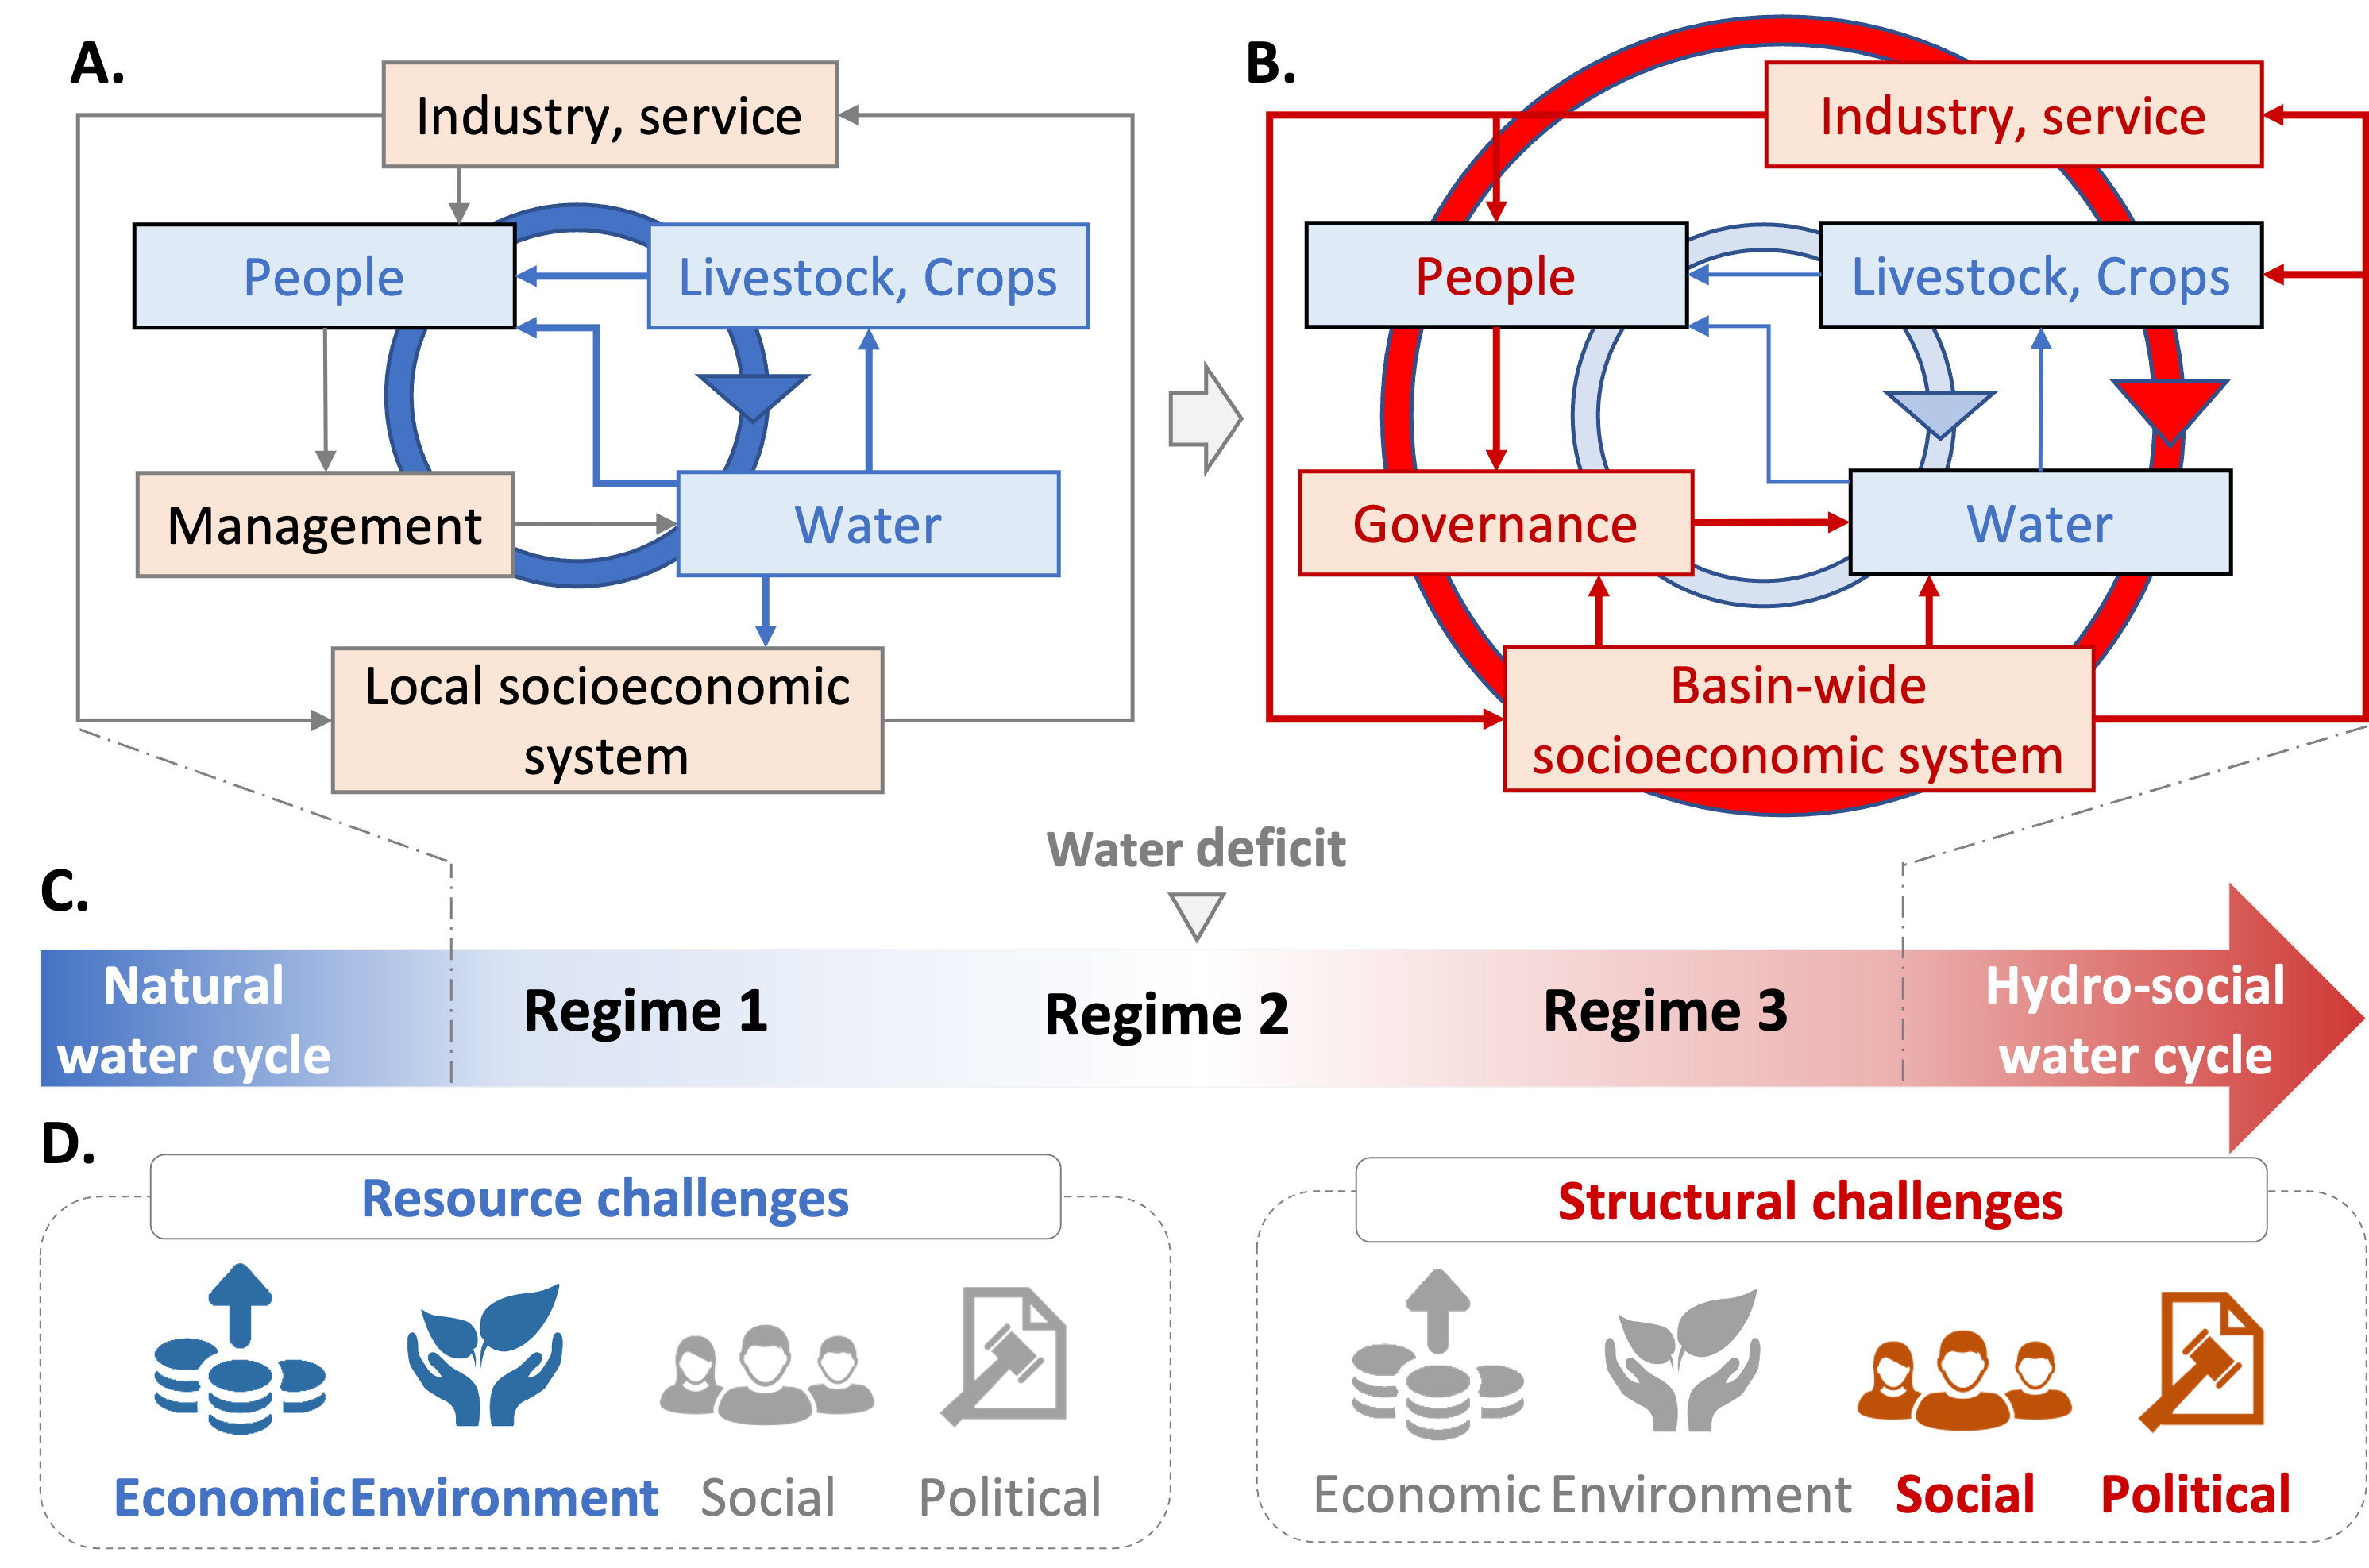
\includegraphics[width=0.9\linewidth]{main/transition.png}
	\caption{
		Transition schema of water governance during transformation towards a hydrosocial water cycle. Blue pathways are dominated by natural water cycle while red pathways are dominated by socio-economic feedbacks. There is a transformation towards the hydrosocial water cycle where red loop increases.
		\textbf{A. Early phase.} As socio-economic systems develop, industry and services gradually demand increasing amounts of water; at the same time, increasing social organization and technological capacity allow people to manage water resources more intensively, including intensive intervention in the natural water cycle.
		\textbf{B. Late phase} With further developed and economically efficient industries and services, trade-offs between provisioning-purpose and non-provisioning water use become prominent. Rather than being determined by local socio-economic systems, water withdraws and management are scaled up to the entire basin.
		Thus, \textbf{C. Transformation from a natural water cycle towards the hydro-social water cycle} occurs in paralleled with a transformation towards a hydrosocial water cycle. This is generally distinguished when water resource limits are reached. The three water governance regimes seen in the YRB are identified along this transition (Regime 1: massive supply regime, Regime 2: purpose-focused regime, Regime 3: many-sided governance regime).
		\textbf{D. Water governance challenges} Through the transitional regimes, water governance faces primarily economic and environmental challenges in the early phase and social and policy challenges in the late phase.
	}
	\label{fig:summary}
\end{figure*}

% 我们为的研究结果表明,黄河流域能被识别为三个明显的稳态。
Our results show that there have been three distinct but sequential governance regimes within the YRB (Figure~\ref{fig:phases}): a massive supply regime (1965-1978), a purpose-focused regime (1979-1993) and a many-sided governance regime (1994-2013). Shifts between these regimes were caused by different environmental, economic, social or political drivers (Figure~\ref{fig:Causes}).
% 值得注意的是,这些多方面的变化随着流域逐步迈向水-社会循环的过程中逐步发生的,且在早期主要带来经济、环境方面的挑战,而后期则带来社会和政策方面的挑战。
It is important to note that each regime occurred gradually, with multifaceted causes, as the basin moves towards a hydrosocial water cycle.
The challenges were primarily economic and environmental at the beginning of the YRB's water governance trajectory and social and policy-related towards the end (Figure~\ref{fig:summary}).

% 第一种时期(1965-1978年),流域经济以农业为主,自然水资源相对丰富,用水治理倾向于为农业提供更多的资源。
During the massive supply regime (1965-1978), the basin economy was mainly dependent on the agriculture and natural water resources were relatively abundant (\textit{SI Appendix} Figure S5); water governance thus tended to supply more resources for agriculture (e.g. by construction of reservoirs and channels).
% 因为此时社会经济对自然水循环的影响尚且有限,几乎没有保护政策的治理体系鼓励在需供水的地区进行无节制的取水和蓄水,而很少考虑流域的社会公平。
Due to the limited effects of socio-economic feedbacks on this regime, water governance had few protective policies, assumed an unlimited water supply, and took little consideration of the impacts of water use on social equity and the environment
\cite{zhouDecelerationChinahuman2020}.
% 近80%的地表水用于供应,黄河在稳态的后半段干涸了.
Since nearly 80\% of surface water was used (mainly for provisioning purposes), the Yellow River dried up during the second half of the regime (\textit{SI Appendix} Figure S7).
% 随着干旱化的日益严重,造成了湿地萎缩、生物多样性下降等生态问题,呈现出巨大的环境危机。
Ecological issues, such as wetlands shrinkage and declines in biodiversity, emerged as the drying up became more and more serious, leading a huge social-ecological crisis and a significant challenge to existing modes of water governance rigorously
\cite{wohlfartRiverBasinCourse2016}.

% “目的转轨”的开始恰逢中国的“改革开放”,巨大的社会转型使得新兴工业和服务业打破了农业的主导地位,开始争夺水资源。
The start of the purpose-focused regime (1978) coincided with Chinese ``reform and opening-up''.
This huge social transformation led to the emergence of industry and services, broke the dominance of agriculture, and resulted in higher competition for water use (Figure~\ref{fig:Causes} and \textit{SI Appendix} Fig. S8).
% 面对遗留的环境问题和全新的经济挑战,黄河水利委员会进行了改组,接到水利部(原水电部)的指示,恢复和加强黄河水利委员会的水文、流域管理工作。
In the face of ongoing environmental challenges and new economic challenges, the Yellow River Conservancy Commission (\textit{SI Appendix} Methods S1) underwent a reorganization and received instructions from the Ministry of Water Resources (then called the Ministry of Water Resources and Electric Power) to resume and strengthen work on hydrology and basin management in the YRB
\cite{yellowriverarchivesOrganizationalHistoryYellow2004}.
% 在全国率先出台了新的政策法规(如“87调水方案”)进行调水,成功阻止了灌溉用水量的扩大。
As a result, new policies and regulations (e.g., ``the 87 Water Allocation Scheme'') were introduced in the YRB ahead of the rest of the country to allocate water for stopping the expansion of water consumption
\cite{wangThirtyYearsYellow2018}.

% 直到大约1993年以来,由于社会经济发展后先进技术的广泛应用,水资源利用效率有了显著提高,才出现了下一个政权向全面治理的转变。
The next shift, to the many-sided governance regime, did not occur until a significant increase in water use efficiency in about 1993, overcame some resource limits
\cite{liuWaterconservancyprojects2013}.
% 区域和部门之间在水需求方面的社会经济权衡在这一制度中发挥关键作用,因此水治理需要满足更全面、更有效率的水分配
Since socio-economic trade-offs between water-dependent regions and sectors played a more important role at this regime, water governance had to achieve efficient water allocation while balancing different purposes in the face of limited water supply
\cite{dalinBalancingwaterresource2015}.
% 因此,这一时期开始推广的水权转换项目,可以为其他地区的工业发展节约区域农业用水。
For example, the water rights conversion project that has been popularized during this regime may even save regional agricultural water for industrial developments in other regions, and water transfer has been another huge project to meet water demands within the YRB
\cite{barnettSustainabilityTransferproject2015,yunpengWaterRightTransfer2010}.
% 但是曾帮助流域摆脱环境危机的分水政策却在此时期成为了流域协调和社会公平的桎梏。
On the other hand, the old water policy (e.g., ``the 87 Water Allocation Scheme''), which once helped the YRB resolve its environmental crisis, limited social equity and coordinated allocation under the new regime because of path dependence
\cite{wangThirtyYearsYellow2018}.
% 类似的,此稳态下国家层面的水治理政策都在进行补充或调整,因为这种制度的缺失和社会的不公平正成为流域新的治理挑战。
Many national-level water policies were proposed or adjusted under this regime, as the absence of such policies and social injustice in water use became new structural challenges for governance
\cite{konarExpandingScopeFoundation2019}.

% 一般来说,在向水社会循环的转变过程中,三种治理制度之间的转变是依次发生的。
In general, shifts between the three governance regimes occurred sequentially during a transformation towards the hydrosocial cycle.
% 随着越来越多的人为影响逐渐改变世界,对生态系统动力学从生物物理控制向社会和政治控制的转变可能在社会-生态系统中变得越来越普遍
Transition from biophysical control to social and political control of ecosystem dynamics may become increasingly widespread in social-ecological systems as increasing anthropogenic impacts gradually change the world
\cite{bestPaceHumanInducedChange2020,cummingLinkingeconomicgrowth2018,cummingImplicationsagriculturaltransitions2014}.
Some implications of this kind of change, when accompanied by engineering solutions, have been explored in the Millennium Assessment’s `Technogarden' scenario %! informal citation
\cite{millenniumecosystemassessmentEcosystemshumanwellbeing2005}.
% 流域转向社会-水循环的过程就是典型的社会-生态系统过渡过程,而我们发现在这一过程中水治理的稳态转换呼应了全球水治理面临的两大主要挑战。
The transition regimes identified here echo the two kinds of major water governance challenges globally (resource challenges and structural challenges, Figure~\ref{fig:summary} and \textit{SI Appendix} Fig. S9)
\cite{singhWaterGovernanceChallenges2019,porcherFacingChallengesWater2019}.
% 以水资源短缺和供水困难为代表的资源挑战,主要是未开发和正在开发的流域所面临的,与经济和环境变化密切相关。
Resource challenges, represented as water shortage and water supplying difficulties, are mainly faced by undeveloped and developing basins and are highly related to economic and environmental changes
\cite{allanNavigatingcomplexitiescoordinated2019,florkeWatercompetitioncities2018,liuWaterSustainabilityChina2012}.
% 另一方面,高度控制和发达的流域主要面临结构性挑战,迫切需要在社会政策方面进行协调与合作(如水资源纠纷和缺乏合作治理,特别是跨界河流)。
Alternatively, highly-controlled and developed basins (especially for transboundary rivers) must mainly resolve structural challenges, such as water disputes or lack of equity, and may be in urgent need of novel flexible, efficient sociopolitical governance structures %! Kitroeff citation wrong
\cite{kitroeffThisWarCrossBorder2020,kitroeffThisWarCrossBorder2020,roobavannanRoleSectoralTransformation2017,unep-dhiTransboundaryRiverBasins2016}.
% 非常具有代表性的是,这两类主要挑战在黄河流域快速变迁的过程中先后发生了,伴随着整合了四个维度的(经济、环境、社会、政策)治理稳态的转换。
It is typical that resource challenges and structural challenges have occurred sequentially during the transition of water governance within the YRB.
% 我们的分析表明,过渡的前期常常带来环境和经济层面的治理挑战,而在过渡的后期则主要是社会和政策层面的挑战。
Our analysis thus suggests that the initial phase of transition often leads to resource-focused challenges that result from economic, demographic and environmental change; while later phases are dominated by structural challenges relating to social and political aspects of governance.
% 再一次,我们总结的框架呼应了联合国发展属为水治理提出的四个维度和两大主要问题。
From the perspective of the core dimensions emphasized by the UNDP for water governance, our proposed schema connects governance challenges and the transformation of large river basins towards a hydrosocial water cycle.

% 随着河流流域在不同制度之间的过渡而发生的升级过程也带来了额外的挑战。在经济力量的影响下,水资源利用逐渐从一个地方性的问题转变为国家或国际的问题,大型河流流域成为生态系统服务、经济发展和人类福祉的重要来源。
Additional challenges are raised by the process of upscaling that occurs as river basins transition between regimes. Under the influence of economic forces, water use gradually changes from being a primarily local concern to becoming a national or international concern, with large river basins being critical sources of ecosystem services, economic development, and human wellbeing.
% 例如黄河小浪底调水调沙的生态系统治理需要造成下游河道迅速下切,使农民长期无法从河道中取到灌溉水资源。
For example, the requirement in the ecological system management of water and sediment diversion in the Xiaolangdi Dam of the Yellow River leads to rapid cutting of the downstream river, which makes it impossible for farmers to get irrigation water resources for a long time
\cite{kongEnvironmentalimpactassessments2017}.
% 通过升级过程成功地引导水况过渡,需要在治理机制中进行相应的升级,并创建能够调节和管理跨规模效应的更高级别机构。
Successful navigation of water regime transitions through an upscaling process requires a corresponding upscaling in the governance regime and the creation of higher-level institutions that can regulate and manage cross-scale effects
\cite{cummingScalemismatchessocialecological2006}.

\subsection{Implications and future directions} %! limitations
\label{Outlook}

%! How data obtained, how assumptions are made.

% IWGI指数以一种相对简单但全面的方式概括了水管理的过渡制度。
The IWGI index captures the transitional regimes of water governance in a relatively simple but comprehensive way.
% 对科学家和决策者来说,认识到不断变化的治理挑战是重要的,因为发展并不是解决所有与可持续性有关的流域问题的万能药
It is important for scientists and decision makers to recognize the changing governance challenges, because development is not a panacea for all basin issues regarding sustainability.
%\cite{cummingLinkingEconomicGrowth2018, reyersSocialEcologicalSystemsInsights2018}.
% 在一种制度下开发的模型和方法在另一种制度下不一定有用。
Models and approaches developed under one regime are not necessarily useful under a different regime.
% 就当今世界而言,与水有关的挑战仍是我们在实现可持续性方面取得进展的主要差距之一,而发展优先战略在许多地方仍是主导方针,可能不利于改善治理
For today's world, water-related challenges remains one of the major gaps in our progress towards sustainability, while development-first strategies are still a dominant guideline in many places and may be in opposition to improving governance
\cite{xuAssessingprogresssustainable2020,liuAerosolweakenedsummermonsoons2017,greveGlobalassessmentwater2018}.
% 虽然大多数大型河流流域随着发展而在水管理技术和水利用效率方面有所改善,但淡水利用仍被认为正在接近人类-水系统可能崩溃的行星边界
Although most large river basins have shown improvements in water management technologies and water use efficiency along with development, freshwater use is still considered to be approaching planetary boundaries where human-water systems may collapse
\cite{anExploringeffectsGrain2017,degraafEnvironmentalflowlimits2019,hugginssocialecologicaldimensionschanging2020}.
% 总的来说,这种明显的治理失败可能有两个主要原因。
Overall, there are probably two main reasons for this apparent failure of governance.
% 首先,农业灌溉效率的显著提高通常伴随着灌溉面积的重新扩大,导致水资源压力的趋势不减(效率悖论)
First, significant improvement in agricultural irrigation efficiency is usually accompanied by a re-expansion of irrigated area, resulting in an unabated trend of water resources stress (the paradox of efficiency)
\cite{graftonparadoxirrigationefficiency2018}.
% 其次,如果没有成功的治理,以水循环为主导的复杂治理结构可能会导致流域尺度上水资源使用的灵活性降低,破坏社会-生态系统的恢复力
Second, without successful governance, complicated governance structures dominated by hydrosocial water cycles may result in less flexible water use and undermine the resilience of social-ecological systems at a basin scale
\cite{qinFlexibilityintensityglobal2019,leviaHomogenizationterrestrialwater2020,grillMappingworldfreeflowing2019}.
% 从这些角度来看,我们需要更好、更全面的策略来应对治理挑战,因为核心问题是复杂而难以管理的
From these perspectives, we need better and more comprehensive strategies to address governance challenges because the core problems are complex and difficult to manage
\cite{steffenemergenceevolutionEarth2020,muneepeerakulemergenceresilienceselforganized2020,bodinCollaborativeenvironmentalgovernance2017,biermannNavigatingAnthropoceneImproving2012}.
% 更深入地了解包含非线性变化、制度和过渡思想的治理,应该有助于将治理的重点转移到维持流域社会-生态系统的恢复力和提高其可持续性。
A deeper understanding of governance that incorporates ideas of non-liner change, regimes, and transitions should help to shift the focus of governance towards maintaining the resilience of the basin’s social-ecological system and improving its sustainability.
